% https://tex.stackexchange.com/a/420485
\documentclass{beamer}
\usepackage{tikz}
\usetikzlibrary{chains}

\begin{document}

\begin{frame}[fragile] 
  \begin{figure}
    %\centering
    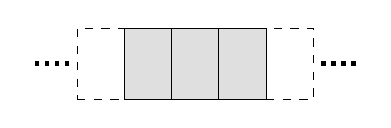
\begin{tikzpicture}[
      node distance = 0pt,
      shorten <>/.style = {shorten <=#1, shorten >=#1},
      start chain = going right,
      box/.style = {shape=rectangle, draw, fill=#1,
      minimum width=6mm, minimum height=9mm, outer sep=0pt,
      node contents={},
      on chain},
      box/.default = none,
      arrow/.style = {draw=blue!60!black, thick, shorten <>=1mm, 
      out=90, in=90, looseness=3,
      -{Straight Barb[bend]}},
      arbox/.style = {inner sep=0pt, minimum size=5pt},
      %crbox/.style = {inner sep=0pt,
      %  node contents={\scriptsize\color{red}$\boldsymbol{\times}$}
      % },
      label distance = -3pt,
      sx/.style = {xshift=#1pt}
    ]
    \node (n0) [box,dashed];
    \foreach \i in {1,2,3}
    \ifnum\i<1
      \node (n\i) [box]
    \else
      \node (n\i) [box=gray!25]
    \fi;
    \node (n14) [box,dashed];
    \draw[ultra thick,dotted,shorten <=1mm]  (n0)  -- + (-9mm,0mm);
    \draw[ultra thick,dotted,shorten <=1mm]  (n14) -- + (+9mm,0mm);
   \end{tikzpicture}
 \end{figure}
\end{frame}

\end{document}
